
\documentclass[12pt]{article}

\usepackage{algorithm}
\usepackage{algpseudocode}
\usepackage{enumitem}
\usepackage[body={7in,9.5in},centering]{geometry}
\usepackage{fancyhdr}
\usepackage{times}
\usepackage{tikz}
\usepackage{hyperref}
\usepackage{graphicx}

\lhead{}
\rhead{}
\renewcommand{\headrulewidth}{3pt}
\lfoot{}
\cfoot{}
\rfoot{}
\pagestyle{empty}

\newcommand*\circled[1]{\tikz[baseline=(char.base)]{
            \node[shape=circle,draw,inner sep=2pt] (char) {#1};}}


\begin{document}
\begin{center}
  \Large
  CIS 675 (Fall 2018) Disclosure Sheet 
\end{center} 
\vspace*{2em}

\noindent
\textbf{\Large Name: \underline{ Wentan Bai }} 


\noindent 
\begin{minipage}[t]{1.0\linewidth}

\begin{minipage}[t]{0.25\linewidth}
\textbf{\Large
  HW \# \underline{ 2 }
} 

\end{minipage} \vspace*{3ex}




\begin{minipage}[t]{.8in}
  \textbf{\circled{Yes} \quad No}
\end{minipage}
\qquad 
\begin{minipage}[t]{5.5in}
  Did you consult with anyone on parts of this assignment, including other students, TAs, or the instructor? 
\end{minipage}
\vspace*{1ex}

\begin{minipage}[t]{.8in}
  \textbf{\circled{Yes} \quad No}
\end{minipage}
\qquad 
\begin{minipage}[t]{5.5in}
  Did you consult an outside source (such as an Internet forum or a
  book other than the course textbook) on parts of this assignment? 
\end{minipage}
\vspace*{1ex}

\noindent
  If you answered \textbf{Yes} to one or more questions, please give the details here: \vspace*{5ex} \par
  I consulted all questions with teaching assistant, Reyhaneh Abdolazimi, to confirm my understanding of all questions are correct. 
  I also consult all questions and extra question with another student, Wentian Bai. For all questions, we discussed our ideas and I finish my algorithms independently. 
  For the extra question, we discussed our understandings and I write my explanation independently.  \vspace*{5ex} \\

  I view some mathematical formulas online.
  \begin{itemize}
    \item \href{url}{https://math.stackexchange.com/questions/1036002/proving-number-of-edges-in-f-n-k} 
   
  \end{itemize}

\vfill
\end{minipage}



\vspace*{40ex}

By submitting this sheet through my Blackboard account, I assert that the information on this sheet is true.

%\vfill

\hfill {\tiny This disclosure sheet was based on one originally designed
  by
  Profs. Royer and Older.}


\pagebreak
\noindent
\large Question 1: \vspace{5mm} \par
\normalsize 
First find the midpoint to divide given array A into two parts. If $midpoint < A[midpoint]$, then recursively find right part. Otherwise, recursively find the left part.
If current midpoint equals to the A[midpoint], it means the given array has an index $i$ such that $A[i] = i$. 
When the length of current array is one and there is not an index $i$ such that $A[i] = i$, just return false.


\begin{algorithm}
\begin{algorithmic}
\Function{find}{int[] $A$, left, right}
  \State \textbf{}$midpoint = left + (right - left) / 2$
  \State \textbf{if} $midpoint == A[midpoint]$:
  \State \hspace{0.8cm}  \textbf{return} $True$
  \State \textbf{if} $length(A) == 1$:
  \State \hspace{0.8cm}  \textbf{return} $False$
  \State \textbf{else if} $midpoint < A[midpoint]$:
  \State \hspace{0.8cm}  \textbf{return find}($A, midpoint \rightarrow right$)
  \State \textbf{else}:
  \State \hspace{0.8cm} \textbf{return find}($A, left \rightarrow midpoint$)
\EndFunction
\end{algorithmic}
\end{algorithm}

\textbf{running time:} \\
The recurrence relation is $T(n) = T(\frac{n}{2}) + O(1)$.\\
Based on Master Method \par
$a = 1$  (only one recursive call will return in each function) \par
$b = 2$  (split the array A into two parts) \par
$d = 0$ (other operations take constant time)\\ 
Thus, $\log_{b}{a} = \log_{2}{1} = 0 = d \Rightarrow T(n) = O({n^0}{\log_{}{n}}) = O(\log_{}{n})$  



\pagebreak
\noindent
\large Question 2: \vspace{5mm} \par
\normalsize 
Divide given array A into two parts and check its midpoint. 
\begin{itemize}
  \item If A[midpoint] is both less than its adjacent values, it is the local minimum. If A[midpoint] is the first or last element of A, only compare with single adjacent element.
  \item If the $A[midpoint] >  A[midpoint+1]$, there must exist a local minimum in the right part. Even if the right part is in decreasing order, the last element also meets the requirements. 
	Thus, recursively call function to find right part of given array. 
  \item Otherwise, recursively find its left part. Even if the left part is in increasing order, the first elelment meets the requirements.
\end{itemize}


\begin{algorithm}
\begin{algorithmic}
\Function{find}{int[] $A$, left, right}
  \State \textbf{if length(A)==1}:
  \State \hspace{0.8cm} \textbf{return} $A[0]$
  \State \textbf{}$midpoint = left + (right - left) / 2$
  \State \textbf{if} $A[midpoint]$ less than its adjacent values:
  \State \hspace{0.8cm}  \textbf{return} $midpoint$
  \State \textbf{else if} $A[midpoint] > A[midpoint + 1]$:
  \State \hspace{0.8cm}  \textbf{return find}($A, midpoint \rightarrow right$)
  \State \textbf{else}:
  \State \hspace{0.8cm} \textbf{return find}($A, left \rightarrow midpoint$)
\EndFunction
\end{algorithmic}
\end{algorithm}

\textbf{running time:} \\
The recurrence relation is $T(n) = T(\frac{n}{2}) + O(1)$.\\
Based on Master Method \par
$a = 1$  (only one recursive call will return in each function) \par
$b = 2$  (split the array A into two parts) \par
$d = 0$ (other operations take constant time)\\ 
Thus, $\log_{b}{a} = \log_{2}{1} = 0 = d \Rightarrow T(n) = O({n^0}{\log_{}{n}}) = O(\log_{}{n})$  


\pagebreak
\large Question 3: \vspace{5mm} \par
\normalsize 
\setlength{\baselineskip}{8mm}
Based on description of HybridSort, there are 3 cases for $n-size$ input.\par 
The first is that the depth of recursion tree is less than r. In this case, this algrothm is the same as MergeSort. Thus, the running time is $O(n\log{}{n})$. \par
The second is the algorithm recurses to a depth of $r$ and all resulting subarrays have size 1. In this case, $\log{}{n} = r$ so the running time is $O(n \cdot r)$. \par
The last is the algorithm recurses to a depth of $r$ and all resulting subarrays have size larger than 1. 
Let $m$ denotes $2^r$.
Since the depth of recursion tree is $r$,  there are the $2^r$ number of resulting subarrays and the size of each resulting subarray is $\frac{n}{2^r}$.
We use InsertionSort to sort each resulting subarry, so the worst running time of each InsertionSort is $(\frac{n}{2^r})^2$.
There are $2^r$ numbers of  resulting subarrays, so the time is $(2^r) \cdot (\frac{n}{2^r})^2 = \frac{n^2}{2^r} $
The merge part is the same as MergeSort and the running time is $O(r \cdot n)$.  \par
When we consider the running time of some algorithms, the time often refers to the worst running time. 
The total time should combine the running time of MergeSort and InsertionSort. Thus, the time is $O(\frac{n^2}{2^r} + r \cdot n)$\\


\pagebreak
\large Question 4: \vspace{5mm}\\
\normalsize 
\setlength{\baselineskip}{8mm}

\underline{Claim:} Based on description, each component of forest is a tree. I need to prove that the number of trees in a forest equals to sum of all nodes minus sum of all edges. \vspace{5mm}\par
\underline{Proof:} \par
If there are a number $c$ of components in forest G, then the sum of all nodes in G is $\sum_{j=1}^{c} {n_j} $, where ${n_j}$ is the number of nodes in its component. \par 
Then the sum of all edges in G is $\sum_{j=1}^{c} {k_j} $, where ${k_j}$ is the number of edges in its component. \par
The sum of all nodes minus sum of all edges is $ n - k = \sum_{j=1}^{c} {n_j} - \sum_{j=1}^{c} {k_j}  = \sum_{j=1}^{c} {(n_j - k_j)}$. 
We know each component of forest is a tree, and for each tree the number of its nodes minus its edges equals to 1, $|V| - |E| = 1$.
Thus, the formula can be transform to $n - k = \sum_{j=1}^{c} {(n_j - k_j)} = \sum_{j=1}^{c} 1 = c$.
Therefore, the claim holds.




\pagebreak
\large Question 5: \vspace{5mm}\\
\normalsize 
\setlength{\baselineskip}{8mm}
\underline{Proof:} \par
No, this algorithm does not always work. Here is a counter example: \\
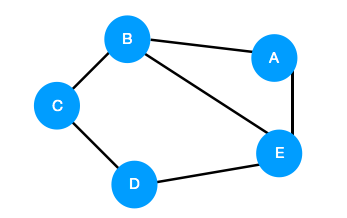
\includegraphics[width=4cm, height=3cm]{undriect} \par
Obviously, the shortest cycle is obviously $A-B-E-A$. However, this is an undirected graph. When we run DFS on the graph and create the DFS tree, it's possible to create a DFS tree as following. \\
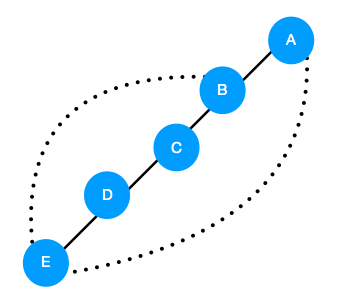
\includegraphics[width=4cm, height=4cm]{tree} \par
Depending on above DFS tree, the shortest cycle is B-C-D-E-B. When we run DFS on the undirected graph, the we do not know the best traversal path. 
If traversal path is in alphabetical order, node E will be prematurely explored. So the back edge (E, A) will appear to be longer than (E, B). \par
Therefore, algorithm does not always work.




\pagebreak
\large \textbf{Extra}:\\ \vspace{5mm}\par
\normalsize 
\setlength{\baselineskip}{8mm}
My algorithm is similar to Breadth-first search. First find all cities from City S with a cable which is less than L. Record the visited edges and cities. 
Then find all cities from visited cities with cables which are less than L. 
If cities or edges are visited, it means there is a shortest path to this cities and stop travers current path because it is not optimal.
Repeat this process untill find City T. \par
In the worst case, we traverse all edges. Therefore, the running time is $O(|E|)$.





 \end{document} 
























